\documentclass[pdftex,abstracton,a4paper]{scrartcl}
\usepackage[T1]{fontenc}
\usepackage[utf8]{inputenc}
\usepackage[ngerman]{babel}
\usepackage[final,colorlinks=true,citecolor=blue,linkcolor=black]{hyperref}
\usepackage[babel,german=quotes]{csquotes}
\usepackage[style=numeric]{biblatex}
\usepackage{graphicx}
\usepackage{awesomebox}
\usepackage{dirtree}
%\usepackage{parskip}
\setlength{\parindent}{0px}
\usepackage{lmodern}

\bibliography{latexlit}
\usepackage[section,nottoc]{tocbibind}

\title{Kurzeinführung Praxissemesterberichtsvorlage}
\author{Sebastian Stigler}

\begin{document}

\maketitle

\tableofcontents

\section{\LaTeX{} Allgemein}

\subsection{Wo bekomme ich \LaTeX{} her?}
\LaTeX wird in Distributionen verbreitet, in denen die einzelnen Pakete passend zueinander gebündelt sind.

Für Windows gibt es entweder \textbf{\TeX{}Live}\autocite{tug:texlive} oder \textbf{MiK\TeX}\footnote{Im Vista-Kompatibilitätsmodus installieren!}\autocite{schenk:miktex}. 
MiK\TeX{} sollte bevorzugt eingesetzt werden, da dort nur ein relativ kleines Basissystem installiert wird und dann erst bei Bedarf einzelne Pakete automatisch nachgeladen werden.

Mac User können \textbf{Mac\TeX}\autocite{tug:mactex} verwenden.

Benutzer von Linux finden i.d.R. in den jeweiligen Repositories der Betriebssysteme ebenfalls \textbf{\TeX{}Live}\autocite{tug:texlive} als Distribution.

\subsection{Welche Editoren kann man verwenden?}

Grundsätzlich kann man jeden UTF-8-fähigen Editor benutzen. Für den Einsteiger hat es sich bewährt, dass man speziell auf \LaTeX{} zugeschnittene Editoren verwendet.

Der für alle Betriebssysteme verfügbare Editor \textbf{\TeX{}maker}\autocite{brachet:texmaker} ist auf jeden Fall empfehlenswert.

Auch der Editor \textbf{\TeX{}Shop}, der bei Mac\TeX{} mit installiert wird, ist brauchbar.

Hingegen ist der Editor \textbf{\TeX{}works}, der bei MiK\TeX{} und \TeX{}Live mit installiert wird, nur sehr rudimentär ausgestattet. 

\warningbox{%
\textbf{UTF-8 und das Literaturverzeichnis}: %
Da das altbekannte \texttt{bibtex}-Programm, %
mit dessen Hilfe man \texttt{*.bib}-Dateien für das %
Literaturverzeichnis in \LaTeX{} vorbereitet, kein UTF-8 % 
unterstützt (und die Vorlage bereits mit dem Programm %
{\texttt{biber}} arbeitet), muss in den Editoren %
der Aufruf für das Programm \textbf{\texttt{bibtex}} %
durch \textbf{\texttt{biber}}%
\footnote{Bei Linux muss das Programm auch noch installiert werden. %
Das Paket heißt \texttt{biber}.} ersetzt werden.%
}   


\subsection{Wie sieht es mit Büchern und Nachschlagewerken aus?}

Als Lernbuch und Arbeitsbuch empfiehlt sich das Buch von Joachim Schlosser (Abbildung~\ref{fig:schlosser}). Hierzu stellt die Bibliothek der Hochschule\footnote{Aus dem interenen WLAN oder per VPN von zuhause.} ebenfalls einen Zugang zu insgesamt ca. 11 Stunden langen Videos\autocite{schlosser:latex_tutorium} zur Verfügung, die auf diesem Buch beruhen.

Eher als Nachschlagewerke eignen sich die beiden Klassiker von Kopka bzw. Mittelbach/Goossens (vgl. Abbildungen~\ref{fig:kopka} bzw. \ref{fig:mittelbach_goossens}).

\begin{figure}[h!tbp]
\centering
\begin{minipage}[b]{0.3\textwidth}
\centering

\includegraphics[width=2.5cm]{images/schlosser_latex_buch}
\caption{\autocite{schlosser:latex_buch}}
\label{fig:schlosser}
\end{minipage}
\hfill
\begin{minipage}[b]{0.3\textwidth}
\centering
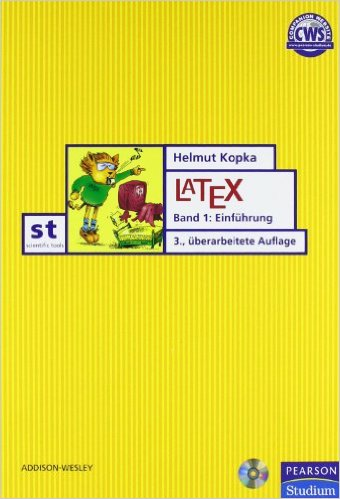
\includegraphics[width=2.5cm]{images/kopka_latex}
\caption{\autocite{kopka:latex}}
\label{fig:kopka}
\end{minipage}
\hfill
\begin{minipage}[b]{0.3\textwidth}
\centering

\includegraphics[width=2.5cm]{images/mittelbach_goossens_latex_begleiter}
\caption{\autocite{mittelbach_goossens:latex_begleiter}}
\label{fig:mittelbach_goossens}
\end{minipage}
\end{figure}

\clearpage
\section{Die Vorlage}

Die Vorlage besteht aus folgenden Dateien:

\dirtree{%
.1 /.
.2 pdf/.
.3 Readme.pdf\DTcomment{dieses Dokument}.
.3 TestDokument\_DE.pdf\DTcomment{das übersetzte Beispieldokument in Deutsch}.
.3 TestDokument\_EN.pdf\DTcomment{das übersetzte Beispieldokument in Englisch}.
.2 readme/.
.3 images/.
.4 kopka\_latex.jpg.
.4 mittelbach\_goossens\_latex\_begleiter.jpg.
.4 schlosser\_latex\_buch.jpg.
.3 infobox.sty.
.3 latexlit.bib.
.3 Readme.tex.
.2 vorlage/.
.3 images/.
.4 ausarbeitung.jpg\DTcomment{nur für das Beispieldokument}.
.4 htw-aalen.pdf.
.4 htw-aalen-en.pdf.
.3 ausarbeitung.cls.
.3 latexlit.bib.
.3 TestDokument.tex\DTcomment{das Beispieldokument}.
}

Um Ihre eigene Arbeit zu erstellen, wechseln Sie bitte in das Verzeichnis
\texttt{vorlage}.
Sie können eine Kopie von \texttt{TestDokument.tex} als Grundlage benutzen.

\subsection{Sprache}
\label{sec:sprache}

Die Vorlage ist zweisprachig verfasst. 
Es ist möglich, die Arbeit in Deutsch als auch in Englisch zu verfassen.
Dafür ist am Anfang von \texttt{TestDokument.tex} folgender Abschnitt zuständig:

\begin{verbatim}
%--- Sprachauswahl
% Erlaubte Werte:
%   \selectlanguage{english}
%   \selectlanguage{ngerman}
\selectlanguage{ngerman}
\end{verbatim}

Wählen Sie einfach die entsprechende Sprache aus.

Folgende Bereiche werden automatisch übersetzt:

\begin{itemize}
  \item Titelseite
  \begin{itemize}
    \item Logo
    \item Dokumenttyp (Praxissemesterberich, Projektarbeit, Bachelorarbeit, Seminararbeit, Masterarbeit)
    \item Studiengang (Informatik, Elektronik, Data Science)
    \item Übergänge zwischen Titel, Firmenname und Student
    \item Betreuer
    \item Einreichdatum
  \end{itemize}
  \item Angaben zur Firma
  \item Eidesstattliche Erklärung
  \item Kurzfassung (nur Überschrift)
  \item Inhalts-, Abbildungs-, Tabellen-, Quelltext-, Abkürzungs- und Literaturverzeichnis
  \item Die Namen an den Nummerierungen für Abbildungen, Tabellen und Quelltext
\end{itemize}

Alles Weitere müssen Sie selbst machen (Kapitelüberschriften und Inhalt).
 
\subsection{Titelseite}
\label{sec:titleseite}
Für die Titelseite müssen Sie folgende Kommandos benutzen, um die entsprechenden Einträge anzupassen und die Titelseite zu erzeugen:

\begin{verbatim}
%--- Art der Arbeit
% Erlaubte Werte:
%   \Praxissemesterbericht
%   \Projektbericht
%   \Bachelorarbeit
%   \Seminararbeit
%   \Masterarbeit

\Praxissemesterbericht

%--- Studiengang:
% Erlaubte Werte:
%   \Informatik
%   \Elektronik
%   \DataScience
\Informatik

\title{Titel der Arbeit}

\author{Jon Doe}
\matrikelnr{12345}

%--- Ist der Erstbetreuer (\examinerA) an der Hochschule ein Professor?
% Erlaubte Werte:
%   \examinerIsAProfessortrue   % Ja
%   \examinerIsAProfessorfalse  % Nein
\examinerIsAProfessortrue   % Ja

%--- Betreuer
\examinerA{Prof.~Dr.~Rainer~Werthebach}
%\examinerB{Prof.~Dr.~Ulrich~Klauck}

%--- Einreichungsdatum
\date{01. Dezember 2016}
\end{verbatim}

\warningbox{\textbf{Hier hat sich etwas im Vergleich zur alten Vorlage geändert!}

Die Art der Arbeit wird direkt mit den Kommandos \texttt{\textbackslash Praxissemsterbericht} o. ä.  geändert. Vergessen Sie bitte nicht den Backslash! Diese Kommandos beinhalten die deutsche und englische Version des Eintrags auf der Titelseite.

Das selbe gilt auch für die Wahl des Studiengangs.

Ferner kann man jetzt auch mit den Kommandos \texttt{\textbackslash
 examinerIsAProfessor\color{blue}true} bzw.\texttt{\textbackslash
 examinerIsAProfessor\color{blue}false} steuern ob für den Erstbetreuer der Text \textit{Betreuender Professor} oder \textit{Betreuender Mitarbeiter} steht. Für den Zweitbetreuer steht in beiden Fällen \textit{Zweitprüfer} auf der Titelseite.}

Und etwas weiter unten im Dokument steht die Anweisung, die Titelseite anzuzeigen:

\begin{verbatim}
%--- Titelseite Anzeigen
\maketitle
\cleardoublepage
\end{verbatim}

\subsection{Angaben zur Firma}
\label{sec:praxisstelle}
Die Firma muss nun als nächstes beschrieben werden:

\begin{verbatim}
%--- Angaben zur Firma
% Auskommentieren, wenn die Arbeit nicht bei einer ext. Firma gemacht wurde.
\companyname{Beispielfirma}
\industrialsector{Beispielbranche}
\department{Beispielabteilung}
\companystreet{Beispielstr. 1}
\companycity{12345 Musterstadt}

%--- Angaben zum Betreuer bei dieser Firma
\advisorname{Name des Betreuers}
\advisorphone{(01234) 567-890}
\advisoremail{name@company.xxx}
\end{verbatim}

Und etwas weiter unten im Dokument:

\begin{verbatim}
%--- Firmendaten Anzeigen
% Auskommentieren, wenn die Arbeit nicht bei einer ext. Firma gemacht wurde.
\makeworkplace
\cleardoublepage
\end{verbatim}

\notebox{Wenn Sie Ihre Arbeit(mit Ausnahme des Praxissemesterberichts) an der
 Hochschule und nicht bei einer externen Firma schreiben, dann kommentieren Sie
 bitte beide Blöcke mit Prozentzeichen aus.} 

\subsection{Eidesstattliche Erklärung und Bestätigung}

Die Erklärung sowie die Bestätigung bedienen sich aus den Einstellungen, die Sie in den Unterabschnitten~\ref{sec:titleseite} bzw. \ref{sec:praxisstelle} gemacht haben, und werden mit dem folgenden Kommando erzeugt:

\begin{verbatim}
%--- Eidesstattliche Erklärung anzeigen
\makeaffirmation
\cleardoublepage
\end{verbatim}

\subsection{Die Kurzfassung}

Hier implementiert die Vorlage die Umgebung \verb+abstract+ mit der Sie die Kurzfassung Ihrer Arbeit schreiben können:

\begin{verbatim}
\begin{abstract}
  Hier kommt Ihre Kurzfassung Ihrer Arbeit hin.
\end{abstract}
\end{verbatim}


\subsection{Inhalts-, Abbildungs-, Tabellen-, Quelltextverzeichnis}

Ihre Arbeit sollte auf jeden Fall ein Inhaltsverzeichnis enthalten (zumal dies mit 
\LaTeX{} in einem Befehl \verb+\tableofcontents+ erledigt ist).

Je nach Bedarf sollte auch ein Abbildungs-, ein Tabellen- und ein Quelltextverzeichnis angelegt werden (so es denn Abbildungen oder Tabellen in Ihrer Arbeit gibt). Hierfür sind folgende Kommandos da:
\begin{itemize}
  \item \verb+\listoffigures+
  \item \verb+\listoftables+
  \item \verb+\listoflistings+ bzw. \verb+\lstlistoflistings+
\end{itemize}

\notebox{Sie könenn ab sofort auch diese Kommandos einfach im \LaTeX{} Dokument stehen lassen. %
Die Verzeichnisse werden nur dann angezeigt, wenn diese auch tatsächlich mit Inhalt gefüllt sind.}



\subsection{Abkürzungsverzeichnis}
Für das Abkürzungsverzeichnis enthält die vorgefertigte Dokumentklasse das Paket
\verb+acronym+. Die Abkürzungen werden dabei in der gleichnamigen Umgebung gesetzt 
und mit dem Kommando \verb+\acro{Referenzname}[Kürzel]{Langform}+ definiert:

\begin{verbatim}
\listofabbreviations
\begin{acronym}[Bsp.]  % Längstes Kürzel in der nachfolgenden
                       % Liste um die Breite der Spalte für die
                       % Abkürzungen zu bestimmen.

\acro{bsp}[Bsp.]{Beispiel}
\end{acronym}
\end{verbatim}

Im Text wird die Abkürzung dann mit \verb+\ac{Referenzname}+ benutzt.
Bei der ersten Benutzung wird dann die Langform mit dem Kürzel in Klammen 
ausgegeben. Bei allen weiteren Benutzungen wird dann nur noch das Kürzel gedruckt. 

\notebox{Das \texttt{\textbackslash listofabbreviations} Kommando beinhaltet das setzen einer Überschrift (inkl. Übersetzung) sowie den Eintrag ins Inhaltsverzeichnis. Auch hier gilt, wie bei
den andernen Verzeichnissen, dass das Abkürzungsverzeichnis nur angezeigt wird, wenn es
mit \texttt{\textbackslash acro} definierte Abkürzungen gibt.}

\subsection{Die übrigen Kapitel}

Sie können nun die übrigen Überschriften aus dem Beispieldokument als Vorlage für Ihre Arbeit benutzen.

Falls Sie aber der Meinung sind, dass eine andere Aufteilung in Ihrem Fall sinnvoller ist, so steht es Ihnen natürlich frei, diese Aufteilung abzuändern.

Dies kann z.B. der Fall sein, wenn Sie nicht eine große, sondern viele kleine Aufgaben bekommen haben. Dann kann eine chronologische Beschreibung Ihrer Tätigkeiten besser sein.

\notebox{Im Zweifelsfall halten Sie Rücksprache mit Ihrem Betreuer!}


\subsection{Das Literaturverzeichnis}

Zu wissenschaftlichen Arbeiten gehört unabdingbar ein Verzeichnis der verwendeten Literatur hinzu. Dies wird in \LaTeX{} mittels einer externen Datei mit der Endung \verb+.bib+ und dem Tool \verb+biber+\footnote{Früher wurde \texttt{bibtex} verwendet} eingefügt. 

\notebox{Nur Einträge aus der \texttt{.bib}-Datei, die zitiert wurden, erscheinen auch im Literaturverzeichnis! Mit dem \LaTeX{}-Kommando \texttt{\textbackslash{}nocite\{...\}} kann man auch Einträge sichtbar machen, die nicht zitiert wurden.}

In der Präambel gibt man mit \verb+\bibliography{latexlit}+ an, dass man die Datei \\\verb+latexlit.bib+ verwenden möchte. Mit  \verb+\autocite{...}+ zitiert man einen Eintrag im Text und schließlich benutzt man im Appendix das Kommando \verb+\printbibliography+, um das Literaturverzeichnis zu erstellen.

\section{Erstellen des PDF-Dokuments}

Heißt Ihre \LaTeX{}-Datei \verb+Praxissemesterbericht.tex+, so erzeugt die folgene Befehlssequenz das PDF Dokument:

\begin{verbatim}
pdflatex Praxissemesterbericht.tex
biber Praxissemesterbericht
pdflatex Praxissemesterbericht.tex
pdflatex Praxissemesterbericht.tex
\end{verbatim}

Der erste Aufruf von \texttt{pdflatex} übersetzt dabei das Dokument, sammelt aber zunächst nur die Überschriften, Referenzen und benutzten Zitate auf, um diese darauf vorzubereiten in den entsprechenden Verzeichnissen bzw. Textstellen benutzt zu werden.

Aus diesen Informationen stellt \texttt{biber}, zusammen mit der benutzten \texttt{.bib}-Datei, die notwendigen Einträge für das Literaturverzeichnis zusammen und berechnet die Textmarken, die im Text für die Zitate benutzt werden sollen.

\textbf{Bitte beachten Sie, dass das Kommando \texttt{biber} nur den Basisnamen der \texttt{.tex}-Datei \textit{ohne Endung} als Parameter benutzt!}

Der nachfolgende \texttt{pdflatex}-Aufruf setzt nun, neben dem Text, auch den Inhalt der Verzeichnisse sowie die berechneten Referenzen, Textmarken und Zitate. Dadurch kann es aber vorkommen, dass durch die jetzt längeren Verzeichnisse der nachfolgende Text verschoben wird. Dies hat zur Folge,dass die Seitenzahlen in diesen nicht mehr stimmen. Aus diesem Grund muss \texttt{pdflatex} ein weiteres Mal aufgerufen werden.

\appendix
\printbibliography[heading=bibintoc]
\end{document}

%
% EOF
%

